%\documentclass[12pt,a4paper]{report}
\documentclass[12pt,a4paper,oneside,onecolumn,openright]{book}
% set the document language
\usepackage[italian]{babel}
% set the encoding used by your editor here (default is utf8)
\usepackage[utf8]{inputenc}
\usepackage[T1]{fontenc}

% math packages
\usepackage{amsmath}
\usepackage{amssymb}
% page margins settings
\usepackage[inner=3cm,outer=2.5cm,top=3cm,bottom=2.5cm]{geometry}
%\usepackage{indentfirst}

% other packages
\usepackage[table]{xcolor}
\usepackage{float}
\usepackage{array}
\usepackage{subfigure}
\usepackage{graphicx}
\usepackage{verbatim}
\usepackage{listings}
\usepackage{url}
\usepackage[hidelinks]{hyperref}
% custom colors
\usepackage{color}
\definecolor{light-gray}{gray}{0.96}
\definecolor{cyan}{RGB}{230,230,255}
\definecolor{dkgreen}{rgb}{0,0.6,0}
\definecolor{gray}{rgb}{0.5,0.5,0.5}
\definecolor{mauve}{rgb}{0.58,0,0.82}

% environment for bash code
\lstset{ %
  language=bash,                % the language of the code
  basicstyle=\footnotesize,           % the size of the fonts that are used for the code
  numbers=left,                   % where to put the line-numbers
  numberstyle=\footnotesize,          % the size of the fonts that are used for the line-numbers
  stepnumber=1,                   % the step between two line-numbers. If it's 1, each line 
                                  % will be numbered
  numbersep=5pt,                  % how far the line-numbers are from the code
  backgroundcolor=\color{white},      % choose the background color. You must add \usepackage{color}
  showspaces=false,               % show spaces adding particular underscores
  showstringspaces=false,         % underline spaces within strings
  showtabs=false,                 % show tabs within strings adding particular underscores
%  frame=single,                   % adds a frame around the code
  rulecolor=\color{black},        % if not set, the frame-color may be changed on line-breaks within not-black text (e.g. commens (green here))
  tabsize=2,                      % sets default tabsize to 2 spaces
  captionpos=b,                   % sets the caption-position to bottom
  breaklines=true,                % sets automatic line breaking
  breakatwhitespace=false,        % sets if automatic breaks should only happen at whitespace
  title=\lstname,                   % show the filename of files included with \lstinputlisting;
                                  % also try caption instead of title
  numberstyle=\tiny\color{gray},        % line number style
  keywordstyle=\textbf,          % keyword style
  commentstyle=\color{dkgreen},       % comment style
%  stringstyle=\color{mauve},         % string literal style
  escapeinside={\%*}{*)},            % if you want to add a comment within your code
  morekeywords={*,...,insert,-}               % if you want to add more keywords to the setù
}

% environment for python code
\lstset{
language=Python,
breaklines=true,
breakatwhitespace=true ,
backgroundcolor=\color{light-gray}
}
% appendices package
%\usepackage{appendix}
% set Appendix name used in the toc
%\renewcommand{\appendixtocname}{Appendice}

% interline
\linespread{1.5}
% set numbers for subsections and show them in the toc
\setcounter{tocdepth}{3} 
\setcounter{secnumdepth}{3}

% layout package, style and settings
\usepackage{fancyhdr}
\pagestyle{fancy}

\fancypagestyle{mainmatter}{%		
		\fancyhf{} 
		\fancyhead{}
		\fancyhead[LE,RO]{\thepage}
		\fancyhead[LO]{\footnotesize{\leftmark}}
		\fancyhead[RE]{\footnotesize{\rightmark}}
		\fancyfoot{}
		\addtolength{\headwidth}{\marginparsep}
		\addtolength{\headheight}{2.5pt}
		\renewcommand{\headrulewidth}{0.3pt}
		\renewcommand{\footrulewidth}{0.0pt}
		}
\fancypagestyle{frontmatter}{%
		\fancyhf{} 
		\fancyhead[LE]{\footnotesize{\MakeUppercase{\thepage}}}
		\fancyhead[RO]{\footnotesize{\MakeUppercase{\thepage}}}
		\fancyhead[RE,LO]{}
		\fancyfoot{}
		\addtolength{\headwidth}{\marginparsep}
		\addtolength{\headheight}{2.5pt}
		\renewcommand{\headrulewidth}{0.0pt}
		\renewcommand{\footrulewidth}{0.0pt}
		}
		
		
\usepackage{fancyhdr}
\pagestyle{fancy}
		\fancyhf{} 
		\fancyhead{}
		\fancyhead[LE,RO]{\thepage} 
		\fancyhead[LO]{\footnotesize{\leftmark}}
		\fancyhead[RE]{\footnotesize{\rightmark}}
		\fancyfoot{}
		\addtolength{\headwidth}{\marginparsep}
		\addtolength{\headheight}{2.5pt}
		\renewcommand{\headrulewidth}{0.3pt}
		\renewcommand{\footrulewidth}{0.0pt}

	\graphicspath{ {images/} }
% empty pages have no numbers
\makeatletter
\def\cleardoublepage{\clearpage\if@twoside \ifodd\c@page\else
\hbox{}
  %Potresti voler togliere il commento dalla linea seguente
  %Questa pagina � stata lasciata intenzionalmente vuota.
\thispagestyle{empty}
\newpage
\if@twocolumn\hbox{}\newpage\fi\fi\fi}
\makeatother
%????
%\textwidth=450pt\oddsidemargin=0pt

%\makeatletter 
%  \DeclareRobustCommand*\textsubscript[1]{% 
%    \@textsubscript{\selectfont#1}} 
%  \newcommand{\@textsubscript}[1]{% 
%    {\m@th\ensuremath{_{\mbox{\fontsize\sf@size\z@#1}}}}} 
\makeatother 

\begin{document}

\begin{titlepage}
\begin{center}
{
    \large
    \textbf{Università  degli studi di Modena e Reggio Emilia} \\
   	\textbf{Dipartimento di Scienze Fisiche, Informatiche e Matematiche} \\
    \vspace{\stretch{0.5}}
    \hspace*{0cm} \hrulefill \hspace*{0cm} \\
    \vspace{\stretch{0.5}}
   	\emph{Corso di Laurea in informatica}
    
	  \vspace{\stretch{12}}
  
  
 		\huge{\bf Titolo: prima riga }}\\
		\vspace{3mm}
		{\huge{\bf Seconda riga}}\\
		\vspace{3mm}
		\vspace{3mm}
		{\huge{\bf Terza riga}}\\
		\vspace{3mm}
		\vspace{3mm}
		{\huge{\bf Quarta riga}}\\
		
		\vspace{\stretch{6}}
		\end{center}
		
\vspace{40mm}
\par
\noindent
\begin{minipage}[t]{0.47\textwidth}
{\large{\bf Relatore:\\
Luca Ferretti}}\\ 
\\

\end{minipage}
\hfill
\begin{minipage}[t]{0.47\textwidth}\raggedleft
{\large{\bf Candidato:\\
Fabio Zanichelli}}
\end{minipage}
\vspace{20mm}
\begin{center}
%\rule[0.1cm]{15.8cm}{0.1mm}
\hspace*{0cm} \hrulefill \hspace*{0cm} \\
{\large{\bf 
Anno Accademico 2021/2022}}
\end{center}

\end{titlepage}

\pagestyle{frontmatter}
\frontmatter

% PAGINA VUOTA
%\clearpage\null\thispagestyle{empty}\clearpage
\setcounter{tocdepth}{2}
\tableofcontents

\setlength{\parindent}{12pt}
\setlength{\parskip}{1ex plus 0.5ex minus 0.2ex}
\mainmatter
\pagestyle{mainmatter}



\chapter{Introduzione}
\label{introduzione}

\section{OS Fingerprinting}
\label{citazioni}

L'OS fingerprinting consiste nel rilevare da remoto il sistema operativo di un dispositivo analizzandone i pacchetti inviati. Le differenze di implementazione dello stack TCP/IP, infatti, determinano comportamenti diversi che, analizzati, consentono di ottenere informazioni utili a questo scopo. \\
Il fingerprinting può essere effettuato in due modalità: attiva e passiva. \\ 
Nella prima si analizzano le risposte ricevute in seguito ad alcuni pacchetti inviati; questi sono appositamente costruiti in modo da massimizzare le informazioni che si possono ottenere dalla risposta.
Nella seconda, invece, viene ispezionato il normale traffico del dispositivo target; si tratta quindi di una tecnica meno invasiva e che si espone meno al rischio di essere scoperti.

\section{Obiettivo}
L'obiettivo consiste nell'analizzare le differenze che portano all'individuazione del sistema operativo, e successivamente modificare determinati parametri di quest'ultimo in modo da riuscire ad ingannare i principali strumenti per il fingereprinting.
I risultati ottenuti, quindi, dovranno essere errati e portare all'individuazione di un sistema operativo differente rispetto a quello realmente in uso.\\
Si è proceduto utilizzando un server HTTP, gestendo quindi pacchetti di non cifrati; si è successivamente cercato di effettuare un'analisi sull'handshake TLS, ovvero sullo scambio di messaggi che precede una comunicazione cifrata.

\section{Strumenti e sistemi operativi utilizzati}
Per la realizzazione dell'obiettivo sono stati utilizzati due differenti sistemi operativi: Windows 11 e Kali (una distribuzione Linux basata su Debian).
La motivazione della scelta di questi sistemi risiede nel fatto che Kali sia stato progettato per la sicurezza informatica, e Windows sia il sistema operativo attualmente più utilizzato; per questa ragione, l'individuazione di quest'ultimo (seppur falsificata) desterebbe meno sospetti. 

I tool utilizzati sono stati i seguenti:
\begin{itemize}
	\item \textbf{Nmap}: principale strumento per effettuare fingerprinting attivo tramite l'invio di specifici pacchetti (\textit{probe}) costruiti appositamente per massimizzare le differenze tra i comportamenti dei sistemi operativi. Consente inoltre di effettuare altre operazioni, alcune delle quali fondamentali per il fingerprinting stesso, come ad esempio il port scanning.
	\item \textbf{p0f}: tool per effettuare fingerprinting passivo. Esso analizza solamente i pacchetti ricevuti da una determinata interfaccia o analizza quelli passati tramite un file con estensione pcap. È anche in grado di effettuare fingerprinting a livello 7.
	\item \textbf{Wireshark}: si tratta di uno strumento che permette la visualizzazione dei pacchetti inviati e ricevuti dal dispositivo tramite un'interfaccia grafica. Consente inoltre di filtrare pacchetti sulla base di determinati campi o protocolli utilizzati.
	\item \textbf{Server Apache}: Web server che consente di rispondere alle richieste di tipo HTTP/HTTPS. È stato installato sia su Windows 11 che su Kali per poter effettuare il confronto tra le risposte inviate.
	\item \textbf{Scapy}: libreria Python in grado di inviare pacchetti modificabili in ogni campo. Molto utile il suo utilizzo per quanto riguarda l'invio di pacchetti "patologici" che stimolano risposte utili ai fini del fingerprinting.
	\item \textbf{nftables}: tool per che permette la modifica o il blocco di pacchetti sulla base del loro contenuto negli header.
\end{itemize}

	







\chapter{Esperienza tirocinio sul fingerprinting}

\section{Obiettivo}
L'obiettivo dell'esperienza consisteva nell'analizzare le differenze che portavano all'individuazione del sistema operativo, e successivamente utilizzare le conoscenze acquisite per modificare dei parametri del sistema operativo in modo da riuscire ad ingannare i principali strumenti per il fingereprinting.
I risultati ottenuti da quest'ultimi, quindi, dovevano essere errati e portare all'individuazione di un sistema operativo differente rispetto a quello realmente in uso.\\
La procedura è stata effettuata su server HTTP, ovvero con pacchetti di dati non cifrati; si è successivamente cercato di effettuare un fingerprinting sull'handshake TLS, ovvero sullo scambio di messaggi che precede una comunicazione cifrata.

\section{Strumenti e sistemi operativi utilizzati}
Per la realizzazione dell'obiettivo sono stati utilizzati due differenti sistemi operativi: Windows 11 e Kali (una distribuzione Linux basata su Debian).
La motivazione risiede nel fatto che Windows sia il sistema più diffuso al mondo e quindi un risultato che individui quello come sistema operativo risulti plausibile agli occhi di chi vuole effettuare il fingerptinging.

I tool utilizzati, oltre ai già citati Nmap e p0f, sono stati i seguenti:
\begin{itemize}
	\item \textbf{Wireshark}, per l'analisi dei pacchetti
	\item \textbf{Server Apache} installati su entrambi i sistemi operativi per simulare le risposte
	\item \textbf{Scapy}, una libreria Python in grado di inviare specifici pacchetti modificabili in ogni campo, e di mostrare i quelli ricevuti
	\item \textbf{nftables}, per la parte successiva all'analisi
\end{itemize}






\chapter{Base knowledge}

Per effettuare comunicazioni tramite internet, vi è il bisogno che tutti i dispositivi connessi rispettino determinati meccanismi; questo si rende necessario a causa dell'elevata eterogeneità derivata da hardware e software differenti.
Questi meccanismi, che prendono il nome di \textit{protocolli}, sono strutturati secondo diversi layer (livelli) formando lo stack TCP/IP.  \\
Sebbene l'idea originale (modello ISO/OSI) prevedesse un modello composto da sette livelli, de facto lo schema attualmente in uso ne prevede solamente quattro. Nonostante ciò, nella terminologia informatica la numerazione dei livelli è rimasta quella precedente.
\\
\begin{table}[htb]
	\centering
	\begin{tabular}{| l | c |}
		\hline
		Livello 7 & Applicativo
		\\
		\hline
		Livello 4 & Trasporto
		\\
		\hline
		Livello 3 & Rete
		\\
		\hline
		Livello 2 & Fisico
		\\
		\hline
		
	\end{tabular}
	\caption{Livelli dello stack TCP/IP}
	\label{tab:stack}
\end{table}

\section{Funzionamento dello stack TCP/IP}
Il meccanismo dello stack prevede che ad ogni livello vengano aggiunte al messaggio delle intestazioni (header), a partire dal layer più alto, che verranno valutate dal medesimo livello del ricevente.
Si precisa che l'ordine in cui si valutano gli header dei livelli è inverso rispetto a quello del mittente; il ricevente partirà infatti dal livello più basso.
Questa procedura prende il nome di \textit{incapsulamento} ed è riassunta nella seguente figura:


\begin{figure}[h]
	\centering
	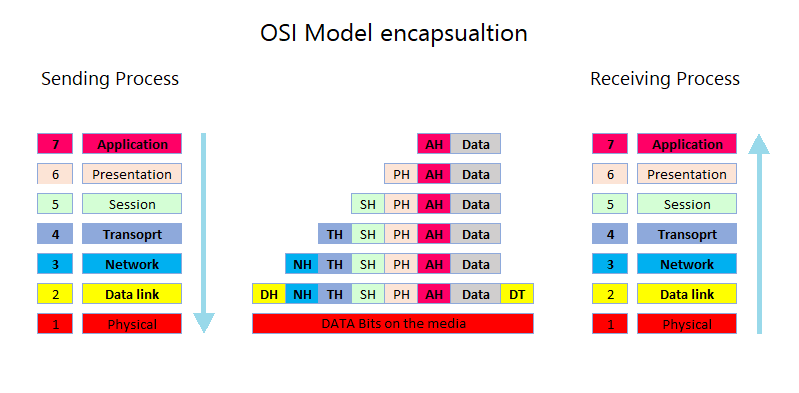
\includegraphics[width=\textwidth]{figures/incapsulamento.png}
	\caption{Incapsulamento nel modello ISO/OSI}
	\label{incapsulamento}
	\cite{incapsulamento}
\end{figure}

\section{Header per il fingerprinting}
Gli header aggiunti ad ogni livello sono formati da vari campi contententi informazioni utili per la comunicazione, e il valore che questi assumono in determinate situazioni è dipendente dal sistema operativo che si sta utilizzando.

Si prenda ad esempio l'header TCP, un protocollo del livello 4 dello stack:\\

\begin{figure}[H]
	\centering
	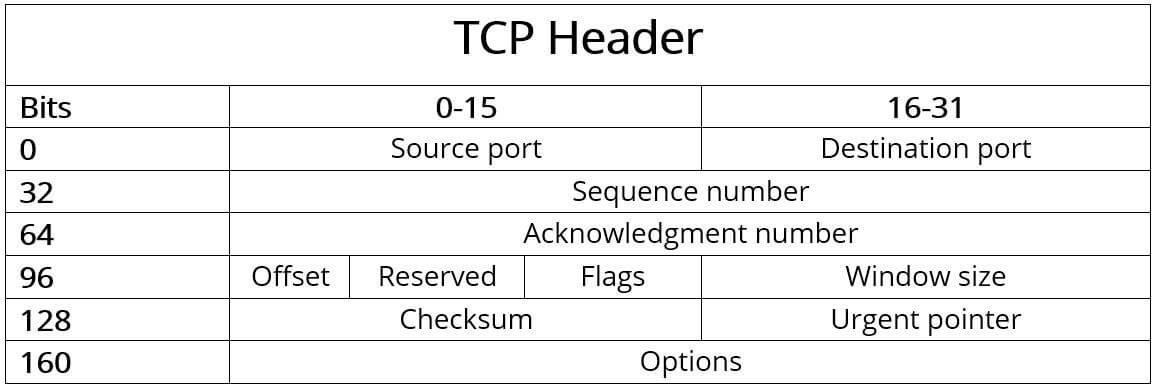
\includegraphics[width=\textwidth]{figures/headerTCP.JPG}
	\caption{Header TCP}
	\label{headerTCP}
	\cite{headerTCP}
\end{figure}

Il campo \textit{option} permette di segnalare al ricevente l'uso di alcune opzioni di comunicazione; il loro supporto e l'effettivo utilizzo, essendo queste facoltative e quindi peculiari di specifici sistemi operativi, rivestono quindi particolare importanza ai fini del fingerprinting.
Esempi analoghi si possono trovare nei protocolli ad ogni livello dello stack, e l'unione delle informazioni acquisite dall'analisi degli header consente di poter individuare con una discreta precisione il sistema operativo del dispositivo target.

% PAGINA VUOTA
%\clearpage\null\thispagestyle{empty}\clearpage
%\appendix
%\appendixpage
%\addappheadtotoc

%\clearpage\null\thispagestyle{empty}\clearpage


%\listoffigures


%\begin{flushleft}
%\bibliographystyle{plain}
%\bibliography{sections/references} 
%\end{flushleft}

\end{document}
